% !Mode:: "TeX:DE:UTF-8:Main"
\documentclass{article}
\usepackage[T1]{fontenc}
\usepackage{AlegreyaSans}
\usepackage{tikzlings}
\usetikzlibrary{patterns,patterns.meta}

\definecolor{europablau}{RGB}{00,33,99}
\newcommand\bearwearlogo{{\sffamily\fontsize{10pt}{12pt}\selectfont
BearWear\raisebox{1ex}[0pt][0pt]{\textcircled{
\begin{tikzpicture}[baseline={(0,0.03)},scale=0.1]
\bear
\end{tikzpicture}}}}}

\tikzset{reverseclip/.style={insert path={
   (current bounding box.south west) --(current bounding box.north west)
 --(current bounding box.north east) --  (current bounding box.south east)
 -- cycle} }}
\begin{document}
\bearwearlogo

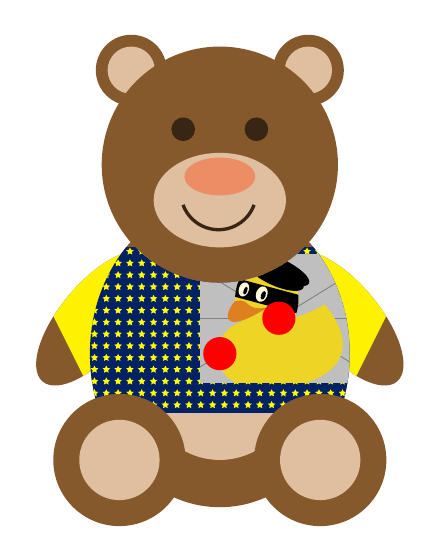
\begin{tikzpicture}[scale=3]
  \bear
  \begin{scope}[even odd rule]
  \coordinate (bearcenter) at (0,0.75);
  \coordinate (bearrightbreast) at (0.25,0.9);
  \clip  (0, 1.55) circle (0.5)[reverseclip];
  \clip  (0.425, 0.3) circle (0.28)[reverseclip];
  \clip  (-0.425, 0.3) circle (0.28)[reverseclip];
  \clip (-1,0.6) --++ (0.45,0)--++(-0.5,1) --cycle[reverseclip] ;
  \clip ( 1,0.6) --++ (-0.45,0)--++(0.5,1) --cycle[reverseclip] ;
  \clip(-1,0.5) rectangle (1,1.2);
  \fill[yellow,rotate around={-50:(0.525,0.9)}](0.525,0.9) ellipse (0.35 and 0.15);
 % \fill[pattern={Stars[points=6,radius=0.5mm,distance=1.5mm]},pattern color=yellow,rotate around={-50:(0.525,0.9)}](0.525,0.9) ellipse (0.35 and 0.15);
%
  \fill[yellow,rotate around={50:(-0.525,0.9)}] (-0.525,0.9) ellipse (0.35 and 0.15);
%  \fill[pattern={Stars[points=6,radius=0.5mm,distance=1.5mm]},pattern color=yellow,rotate around={50:(-0.525,0.9)}] (-0.525,0.9) ellipse (0.35 and 0.15);
  \fill[europablau] (0,0.75) ellipse (0.55 and 0.65);
  \fill[pattern={Stars[points=5,radius=0.5mm,distance=1.5mm]},pattern color=yellow,
  path picture={\node at (bearrightbreast) {\includegraphics[width=2cm,clip,trim=2cm 1cm 2cm
  1cm,page=18]{example-image-duck}};\fill[red] (bearrightbreast) circle(2pt);\fill[red] (bearcenter) circle(2pt); }]
  (0,0.75) ellipse (0.55 and 0.65);
  %\fill[europablau] (0,0.7) ellipse (0.35 and 0.4);
  %\node at (0,0.8){\includegraphics[width=0.5cm,trim=2cm 0.7cm 2cm 0.7cm,clip]{flag_yellow_eps}};
  \end{scope}
\end{tikzpicture}


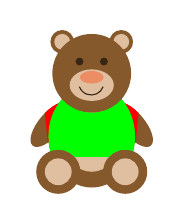
\begin{tikzpicture}
  \bear
  \begin{scope}[even odd rule]

  \clip  (0, 1.55) circle (0.5)[reverseclip]; %head
  \clip  (0.425, 0.3) circle (0.28)[reverseclip]; %right foot
  \clip  (-0.425, 0.3) circle (0.28)[reverseclip]; %left foot
  \clip (-1,0.6) --++ (0.45,0)--++(-0.5,5) --cycle[reverseclip] ; %left arm
  \clip ( 1,0.6) --++ (-0.45,0)--++(0.5,5) --cycle[reverseclip] ; %right arm
  \clip(-1,0.5) rectangle (1,1.2); %overall clip
  \fill[red,rotate around={-50:(0.525,0.9)}](0.525,0.9) ellipse (0.35 and 0.15); %right arm
  \fill[red,rotate around={50:(-0.525,0.9)}] (-0.525,0.9) ellipse (0.35 and 0.15);
  \fill[green] (0,0.75) ellipse (0.55 and 0.65); %body
  %\fill[europablau] (0,0.7) ellipse (0.35 and 0.4); %inner body
  %\node at (0,0.8){\includegraphics[width=0.5cm,trim=2cm 0.7cm 2cm 0.7cm,clip]{flag_yellow_eps}};
  \end{scope}
\end{tikzpicture}


\begin{tikzpicture}
  \bear
  \begin{scope}[even odd rule]

  \clip  (0, 1.55) circle (0.5)[reverseclip]; %head
  \clip  (0.425, 0.3) circle (0.28)[reverseclip]; %right foot
  \clip  (-0.425, 0.3) circle (0.28)[reverseclip]; %left foot
  \clip (-1,0.6) --++ (0.45,0)--++(-0.5,5) --cycle[reverseclip] ; %left arm
  \clip ( 1,0.6) --++ (-0.45,0)--++(0.5,5) --cycle[reverseclip] ; %right arm
  \clip(-1,0.5) rectangle (1,1.2); %overall clip
 % \fill[red,rotate around={-50:(0.525,0.9)}](0.525,0.9) ellipse (0.35 and 0.15); %right arm
 % \fill[red,rotate around={50:(-0.525,0.9)}] (-0.525,0.9) ellipse (0.35 and 0.15);
  \fill[europablau] (0,0.75) ellipse (0.55 and 0.65);
  %\fill[europablau] (0,0.7) ellipse (0.35 and 0.4);
  %\node at (0,0.8){\includegraphics[width=0.5cm,trim=2cm 0.7cm 2cm 0.7cm,clip]{flag_yellow_eps}};
  \end{scope}
\end{tikzpicture}
\end{document}
